%! Tex program = pdflatex
 
\documentclass[UTF8]{ctexart}
\CTEXsetup[format={\Large\bfseries}]{section}
\usepackage{amsmath}
\usepackage{ctex}
\usepackage{array}
\usepackage{ulem}
\usepackage{graphicx}
\usepackage{geometry}
\usepackage{multirow}
\usepackage{subfig}
\usepackage{float}
\usepackage{multicol}
\usepackage{multirow}
\usepackage{indentfirst}
\usepackage{makecell}
\geometry{papersize={21cm,29.7cm}}
\geometry{left=2.54cm,right=2.54cm,top=3.18cm,bottom=3.18cm}
\usepackage{fancyhdr}
\pagestyle{fancy}
\lhead{\today}
\chead{}
\rhead{2020011075}
\lfoot{清华大学}
\cfoot{\thepage}
\rfoot{物理实验B(2)}
\renewcommand{\headrulewidth}{0.4pt}
\renewcommand{\headwidth}{\textwidth}
\renewcommand{\footrulewidth}{0pt}
\usepackage{bm}
\begin{document}
\begin{titlepage}
    \begin{center}
		\quad \\
		\quad \\
        \quad \\
        \quad \\
        \quad \\
        \quad \\
		\kaishu \fontsize{30}{15} 同轴电缆中电磁波的传输\\及金属中超声波的传输
	\end{center}
	\vskip 10cm

    \begin{center}
        \begin{large}
        \begin{tabular}{cc}
        院\qquad 系:& ~~~~~~~~自动化系~~~~~~~~      \\
        \cline{2-2}\\
        班\qquad 级:& 自02班   \\
        \cline{2-2}\\
        学生姓名:& 彭程    \\
        \cline{2-2}\\
        学\qquad 号:&2020011075   \\
        \cline{2-2}\\
        组\qquad 号:& 双四下L    \\
        \cline{2-2}\\
        座~~位~~号:& \# 13    \\
        \cline{2-2}
        \end{tabular}
        \end{large}
        \end{center}

\end{titlepage}
\newpage
\tableofcontents
\newpage
\section{实验名称}
同轴电缆中电磁波的传输及金属中超声波的传输
\section{数据处理}
\subsection{同轴电缆中电磁波的传输}


% Please add the following required packages to your document preamble:
% \usepackage{multirow}
\begin{table}[H]
  \begin{center}
    \begin{tabular}{|c|l|l|}
      \hline
      \multicolumn{1}{|l|}{同轴电缆输出负载}  & 信号幅度 $V_i (mV) $  & 脉冲峰位 $t_i (ns) $   \\ \hline
      \multirow{9}{*}{开路负载}  &     $V_0 =264$       &  $t_0 =10$                 \\
                   &     $V_1 =296$               &  $t_1 =160$               \\
                   &     $V_2 =204$               &  $t_2 =330$                \\
                   &     $V_3 =136$               &  $t_3 =490$                \\
                   &     $V_4 =100$               &  $t_4 =650$                \\
                   &     $V_5 =72$               &   $t_5 =820$                 \\
                   &     $V_6 =52$               &   $t_6 =980$                 \\
                   &     $V_7 =40$               &   $t_7 =1150$                \\ 
                   & $V_8 =32$                   & $t_8 =1310$                   \\\hline
      \multirow{5}{*}{短路负载} & $V_0 =252$ & $t_0 =10$  \\
                       &    $V_1 =-216$     &   $t_1 =310$                \\
                       &    $V_2 =108$     &   $t_2 =620$                \\
                       &    $V_3 =-56$     &   $t_3 =930$                \\
                       &    $V_4 =28$     &   $t_4 =1240$                \\ \hline
      \multirow{2}{*}{匹配负载} & $V_0 =264$  & $t_0 =12$ \\
                       &     $V_0 =196$               &      $t_0 =156$     \\ \hline
      \end{tabular}
  \end{center}
\end{table}

下面分别利用各种负载下的数据计算电缆长度(吸收系数 $\alpha$),并附其波形示意图(黄色:输入
端;蓝色:输出端):

\subsubsection{开路负载}
\begin{figure}[H]
  \centering
  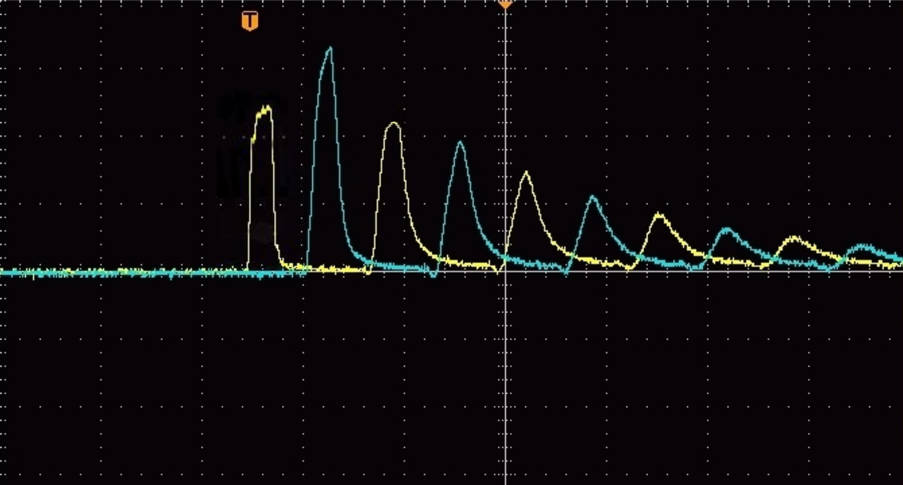
\includegraphics[scale=0.22]{1.jpg}
  \caption{开路负载波形示意图}
  \label{fig:my_label}
\end{figure}

由线性拟合得到:
$$
\delta t=164.17 n s
$$

故有:
$$
l=v \delta t=2 \times 10^{8} \times 164.17 \times 10^{-9}=32.83\mathrm{~m}
$$

对于 $\alpha$, 已知: $V_{l}=V e^{-\alpha l}$, 两边取对数得到: $\ln \left(V_{l}\right)=\ln (V)-\alpha l$, 故可做线性拟合: 拟合得到

$$
\alpha=9.80 \times 10^{-3} \mathrm{~m}^{-1}
$$

拟合曲线如下所示:

\begin{figure}[H]
  \centering
  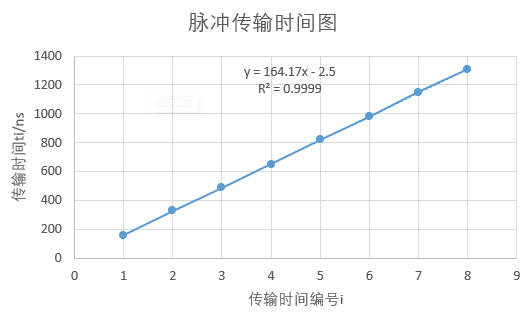
\includegraphics[scale=0.4]{图表1.jpg}
  \caption{开路负载脉冲传输时间图}
  \label{fig:my_label}
\end{figure}


\begin{figure}[H]
  \centering
  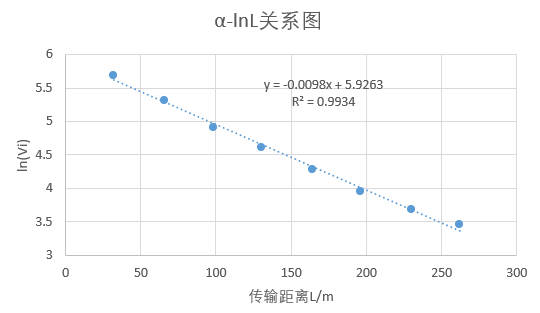
\includegraphics[scale=0.4]{图表2.jpg}
  \caption{开路负载$\alpha-lnL$关系图}
  \label{fig:my_label}
\end{figure}

\subsubsection{短路负载}
\begin{figure}[H]
  \centering
  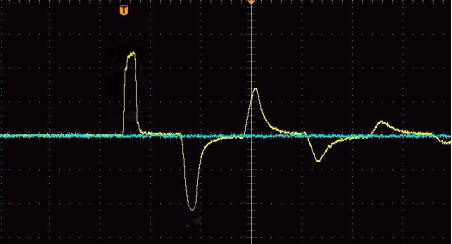
\includegraphics[scale=0.45]{2.jpg}
  \caption{短路负载波形示意图}
  \label{fig:my_label}
\end{figure}

同样, 由线性拟合得到:
$$
\delta_t=154 n s
$$

故有:
$$
l=v \delta t=2 \times 10^{8} \times 128.2 \times 10^{-9}=30.80 \mathrm{~m}
$$

拟合曲线如下所示:


\begin{figure}[H]
  \centering
  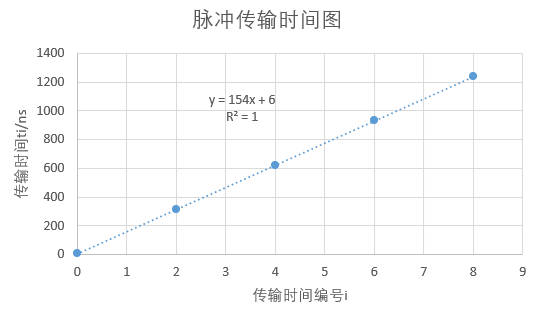
\includegraphics[scale=0.4]{图表3.jpg}
  \caption{短路负载拟合图像}
  \label{fig:my_label}
\end{figure}


\subsubsection{匹配负载}
\begin{figure}[H]
  \centering
  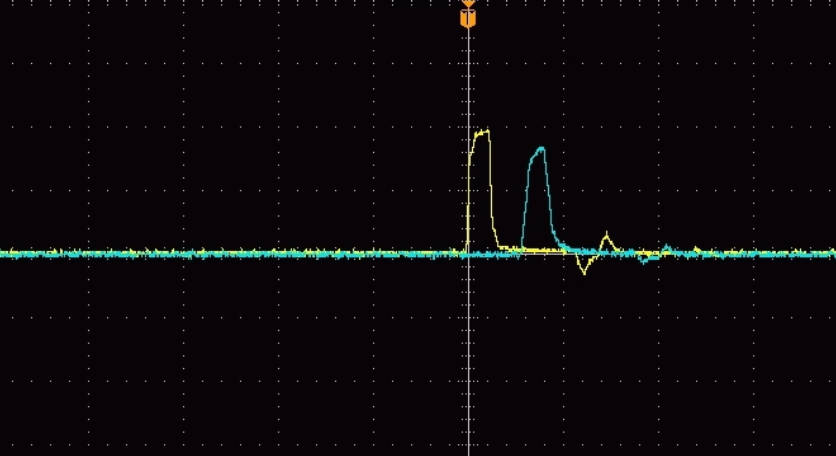
\includegraphics[scale=0.26]{3.jpg}
  \caption{匹配负载波形示意图}
  \label{fig:my_label}
\end{figure}

直接计算可得:
$$
l=\left(t_{1}-t_{0}\right) v=28.8 m
$$



\subsection{金属中超声波的传输}

\subsubsection{声速测量}

\noindent 得到的数据表格如下所示:

\begin{center}
  
\begin{tabular}{|l|l|l|l|}
  \hline \multicolumn{2}{|c|}{ 直探头–纵波 } & \multicolumn{2}{|c|}{ 斜探头–横波 } \\
  \hline 底面回波峰位 $\left(t_{2} / \mu s\right)$ & 表面回波峰位 $\left(t_{1} / \mu s\right)$ & R1 弧面回波峰位 $\left(t_{R 1} / \mu s\right)$ & R2 弧面回波峰位 $\left(t_{R 1} / \mu s\right)$ \\
  \hline $20.00$ & $0.80$ & $25.20$ & $44.40$ \\
  \hline
\end{tabular}
\end{center}

\noindent 1. 利用直探头测量试样中纵波声速 $c_{l}$

$$
\begin{gathered}
c_{l}=\frac{2 H}{t_{2}-t_{1}}=\frac{2 R_{2}}{t_{2}-t_{1}}=6250 \mathrm{~m} / \mathrm{s}
\end{gathered}
$$

\noindent 2. 利用 $45^{\circ}$ 斜探头测量试样中横波声速 $c_{s}$

$$
\begin{gathered}
c_{s}=\frac{2 H}{t_{2}-t_{1}}=\frac{2\left(R_{2}-R_{1}\right)}{t_{2}-t_{1}}=3125 \mathrm{~m} / \mathrm{s}
\end{gathered}
$$

\noindent 3. 利用声速计算样块的杨氏模量和泊松系数

已知测试样密度: $\rho=2700 \mathrm{~kg} / \mathrm{m}^{3}$ (铝)

可知:
$$
T=\frac{c_{l}}{c_{s}}=2.00
$$

则杨氏模量为
$$
E=\frac{\rho c_{s}^{2}\left(3 T^{2}-4\right)}{T^{2}-1}=7.03 \times 10^{10} \mathrm{~Pa}
$$

Poisson 系数为
$$
\sigma=\frac{T^{2}-2}{2\left(T^{2}-1\right)}=0.33
$$

\subsubsection{表面波的实验} 

\noindent 得到的数据表格如下所示:

\begin{center}
\begin{tabular}{|l|l|l|}
  \hline \multicolumn{3}{|c|}{ 可变探头–表面波 } \\
  \hline 探头角度 $\left({ }^{\circ}\right)$ & 探头位置 $\left(l_{E G} / m m\right)$ & 表面波回波 延时 $(\Delta t / \mu s)$ \\
  \hline 60 & $95.0$ & $65.20$ \\
  \hline 探头移动距 & 表面波回波 & 表面波回波 \\
  离 $\left(l_{E I} / m m\right)$ & 峰位 $\left(t_{2} / \mu s\right)$ & 峰位 $\left(t_{1} / \mu s\right)$ \\
  \hline $10.0$ & $71.60$ & $65.20$ \\
  \hline
\end{tabular}
\end{center}


\noindent 1. 固定法测量表面波波速

$$
c_{R}=\frac{2 l_{E G}}{\Delta t}=\frac{2 \times 30 \mathrm{~mm}}{22 \mu \mathrm{s}}=2.91 \times 10^{3} \mathrm{~m} / \mathrm{s}
$$

\noindent 2.移动法测量表面波波速

$$
c_{R}=\frac{2 l_{E I}}{t_{2}-t_{1}}=\frac{2 \times 35 \mathrm{~mm}}{77 \mu \mathrm{s}-52 \mu \mathrm{s}}=3.13 \times 10^{3} \mathrm{~m} / \mathrm{s}
$$

\subsubsection{超声波探测缺陷}  

\noindent 得到的数据表格如下所示:

\noindent 扩散角测量数据记录:

\begin{center}
\begin{tabular}{|c|c|c|c|c|c|}
  \hline \multicolumn{3}{|c|}{ 直探头-扩散角(以 $\mathrm{B}$ 为测量点) } & \multicolumn{3}{|c|}{ 斜探头-扩散角 (以 B 为测量点) } \\
  \hline$x_0$ & $x_1$ & $x_2$ & $x_B$ & $x_1$ & $x_2$ \\
  \hline $52.0 \mathrm{~mm}$ & $59.0 \mathrm{~mm}$ & $47.0 \mathrm{~mm}$ & $84.0\mathrm{~mm}$ & $89.0 \mathrm{~mm}$ & $79.0 \mathrm{~mm}$ \\
  \hline
  \end{tabular}
\end{center}

\noindent  缺陷测量数据记录:

\begin{center} 
\begin{tabular}{|c|c|c|c|c|}
  \hline \multicolumn{2}{|c|}{ 直探头测缺陷 $\mathrm{C}$} & \multicolumn{3}{|c|}{ 斜探头测量缺陷 $\mathrm{D}$ 的位置 } \\
  \hline 底面波 $\left(t_{H}-t_{1}\right)$ & 缺陷波 $\left(t_{C}-t_{1}\right)$ & $x_{A} / t_{A}$ & $x_{B} / t_{B}$ & $x_{D} / t_{D}$ \\
  \hline $20.80 \mu \mathrm{s}$ & $16.00 \mu \mathrm{s}$ & $25.0 \mathrm{~mm} / 22.40 \mu \mathrm{s}$ & $84.0 \mathrm{~mm} / 50.00 \mu \mathrm{s}$ & $117.0 \mathrm{~mm} / 31.60 \mu \mathrm{s}$ \\
  \hline
  \end{tabular}
\end{center}


\noindent 1. 直探头声束扩散角的测量
可知:
$$
\theta=2 \tan ^{-1} \frac{x_{1}-x_{2}}{2 H_{B}}=2 \times 6.84^{\circ}=13.68^{\circ}
$$

\noindent 2. 斜探头声束扩散角的测量

可知折射角:
$$
\beta=\arctan \left(\frac{\left(x_{B}-x_{A}\right)-\left(L_{B}-L_{A}\right)}{H_{B}-H_{A}}\right)=44.0^{\circ}
$$

以 B 为测量点, $L=H_{B}/cos\beta$, 故有
$$
\theta=2 \tan ^{-1}\left(\frac{x_{1}-x_{2}}{2 L}(\cos \beta)^{2}\right)=4.26^{\circ}
$$

\noindent 3. 直探头测量缺陷深度

易知, 由于波的传播速度相同, 应有:

$$
\begin{gathered}
\frac{l_{c}}{l}=\frac{t_{C}-t_{1}}{t_{H}-t_{1}}=0.769 \\
l_{c}=l \times 0.769=R_{2} \times 0.769=46.14 \mathrm{~mm}
\end{gathered}
$$

所以 $\mathrm{C}$ 的高度 $H_{C}$ 为:

$$
H_{C}=l-l_{c}=R_{2}-l_{c}=13.86 \mathrm{~mm}
$$

\noindent 4.斜探头测量缺陷位置

由上述计算可知:折射角 $\beta=44.0^{\circ}$;

若斜探头传输延迟时间为 $\delta_t$, 则:
$$
\begin{aligned}
&H_{A} / \cos \beta=\left(t_{A}-\delta_t\right) c_{S} / 2 \\
&H_{B} / \cos \beta=\left(t_{B}-\delta_t\right) c_{S} / 2
\end{aligned}
$$

由此可知:
$$
\begin{gathered}
\delta t=\frac{H_{B} t_{A}-H_{A} t_{B}}{H_{B}-H_{A}}=4.00 \mu \mathrm{s} \\
H_{D}=\cos \beta\left(t_{D}-\delta t\right) c_{S} / 2=31.02 m m
\end{gathered}
$$

$$
L_D=\tan{\beta}\times\left(H_A-H_D\right)+X_A-X_D+L_A=
$$

又易知:
$$
\begin{aligned}
\tan \beta &=\frac{\Delta+x_{A}-L_{A}}{H_{A}} \\
\Delta &=10.31 \mathrm{~mm}
\end{aligned}
$$

故由于刻度选择和探头真实出射所带来的偏移为 $10.31 \mathrm{~mm}$; 由此得到:
$$
L_{D}=x_{D}+\Delta-H_{D} \tan \beta=117 m m+10.31 m m-31.02 m m \times 0.966=97.34 m m
$$

故 $\mathrm{D}$ 的深度 $H_{D}$ 为 $31.02 \mathrm{~mm}, \mathrm{D}$ 的边距 $L_{D}$ 为 $97.34 \mathrm{~mm}$ 


\section{思考题}
\subsection{同轴电缆思考题}
\noindent \textbf{1. 在测量过程中,如何定位光标更加准确?}

在测量时间时,时间光标对准波峰位置的最高点测量;在测量幅度时,幅度光标和波峰的最高
点对齐,并在抖动存在时统一选择抖动的最高点或是最低点为对齐位置。

\noindent \textbf{2. 如何减小或消除延长线的影响}

找到一根长度已知的同轴电缆,使用同样的延长线进行测量,可计算标准值和测量值的差得到
$\delta_l$,从而作为测量的修正,将本次实验测量的结果加上 $\delta_l$ 即可一定程度上消除延长线影响。

\noindent \textbf{3. 如何提高测量 $\tau$ 的精度}

在测量时,增大示波器的 scale,选取既能清晰观察波形又能更为精确的分度值。

\noindent \textbf{4. 三种测量同轴电缆长度的方法,哪一种更加可靠?为什么?}

开路负载更可靠。因为开路负载反射系数最大为 1,得到的反射波峰最多也最清晰,测量误差更
小,且由于反射波数量更大,数据量的增加同样减小了随机误差。两种方法不确定度都较开路更大。

\subsection{超声波思考题} 

\noindent \textbf{1. 在表面波测量过程中,固定法和移动法哪一种测得的结果更加准确?为什么?}

用移动法测得的表面波声速更准确可靠,由于固定法中标定位置时对探头位置的估计是很不准
确的,移动法可以消除信号发生器到探头之间的距离估计误差。


\section{实验总结}

这次实验的实验原理比较复杂,在预习过程中我遇到了很大的困难,也有很多没有看懂的地方。在老师的讲解之下,我的大部分问题得到了解答,也增加了我的物理知识,很有收获。

这次实验中,我对波的性质有了更深入的了解,对波的反射和折射性质有了更好的理解,并且在老师的讲解中知道了很多波的应用。尤其在第二个实验中,我第一次了解到表面波,还掌握了一种由已知物体缺陷进行定标测量新的缺陷的位置的方法。

最后,感谢老师对我们的悉心指导!

\section{原始数据}

\begin{figure}[H]
  \centering
  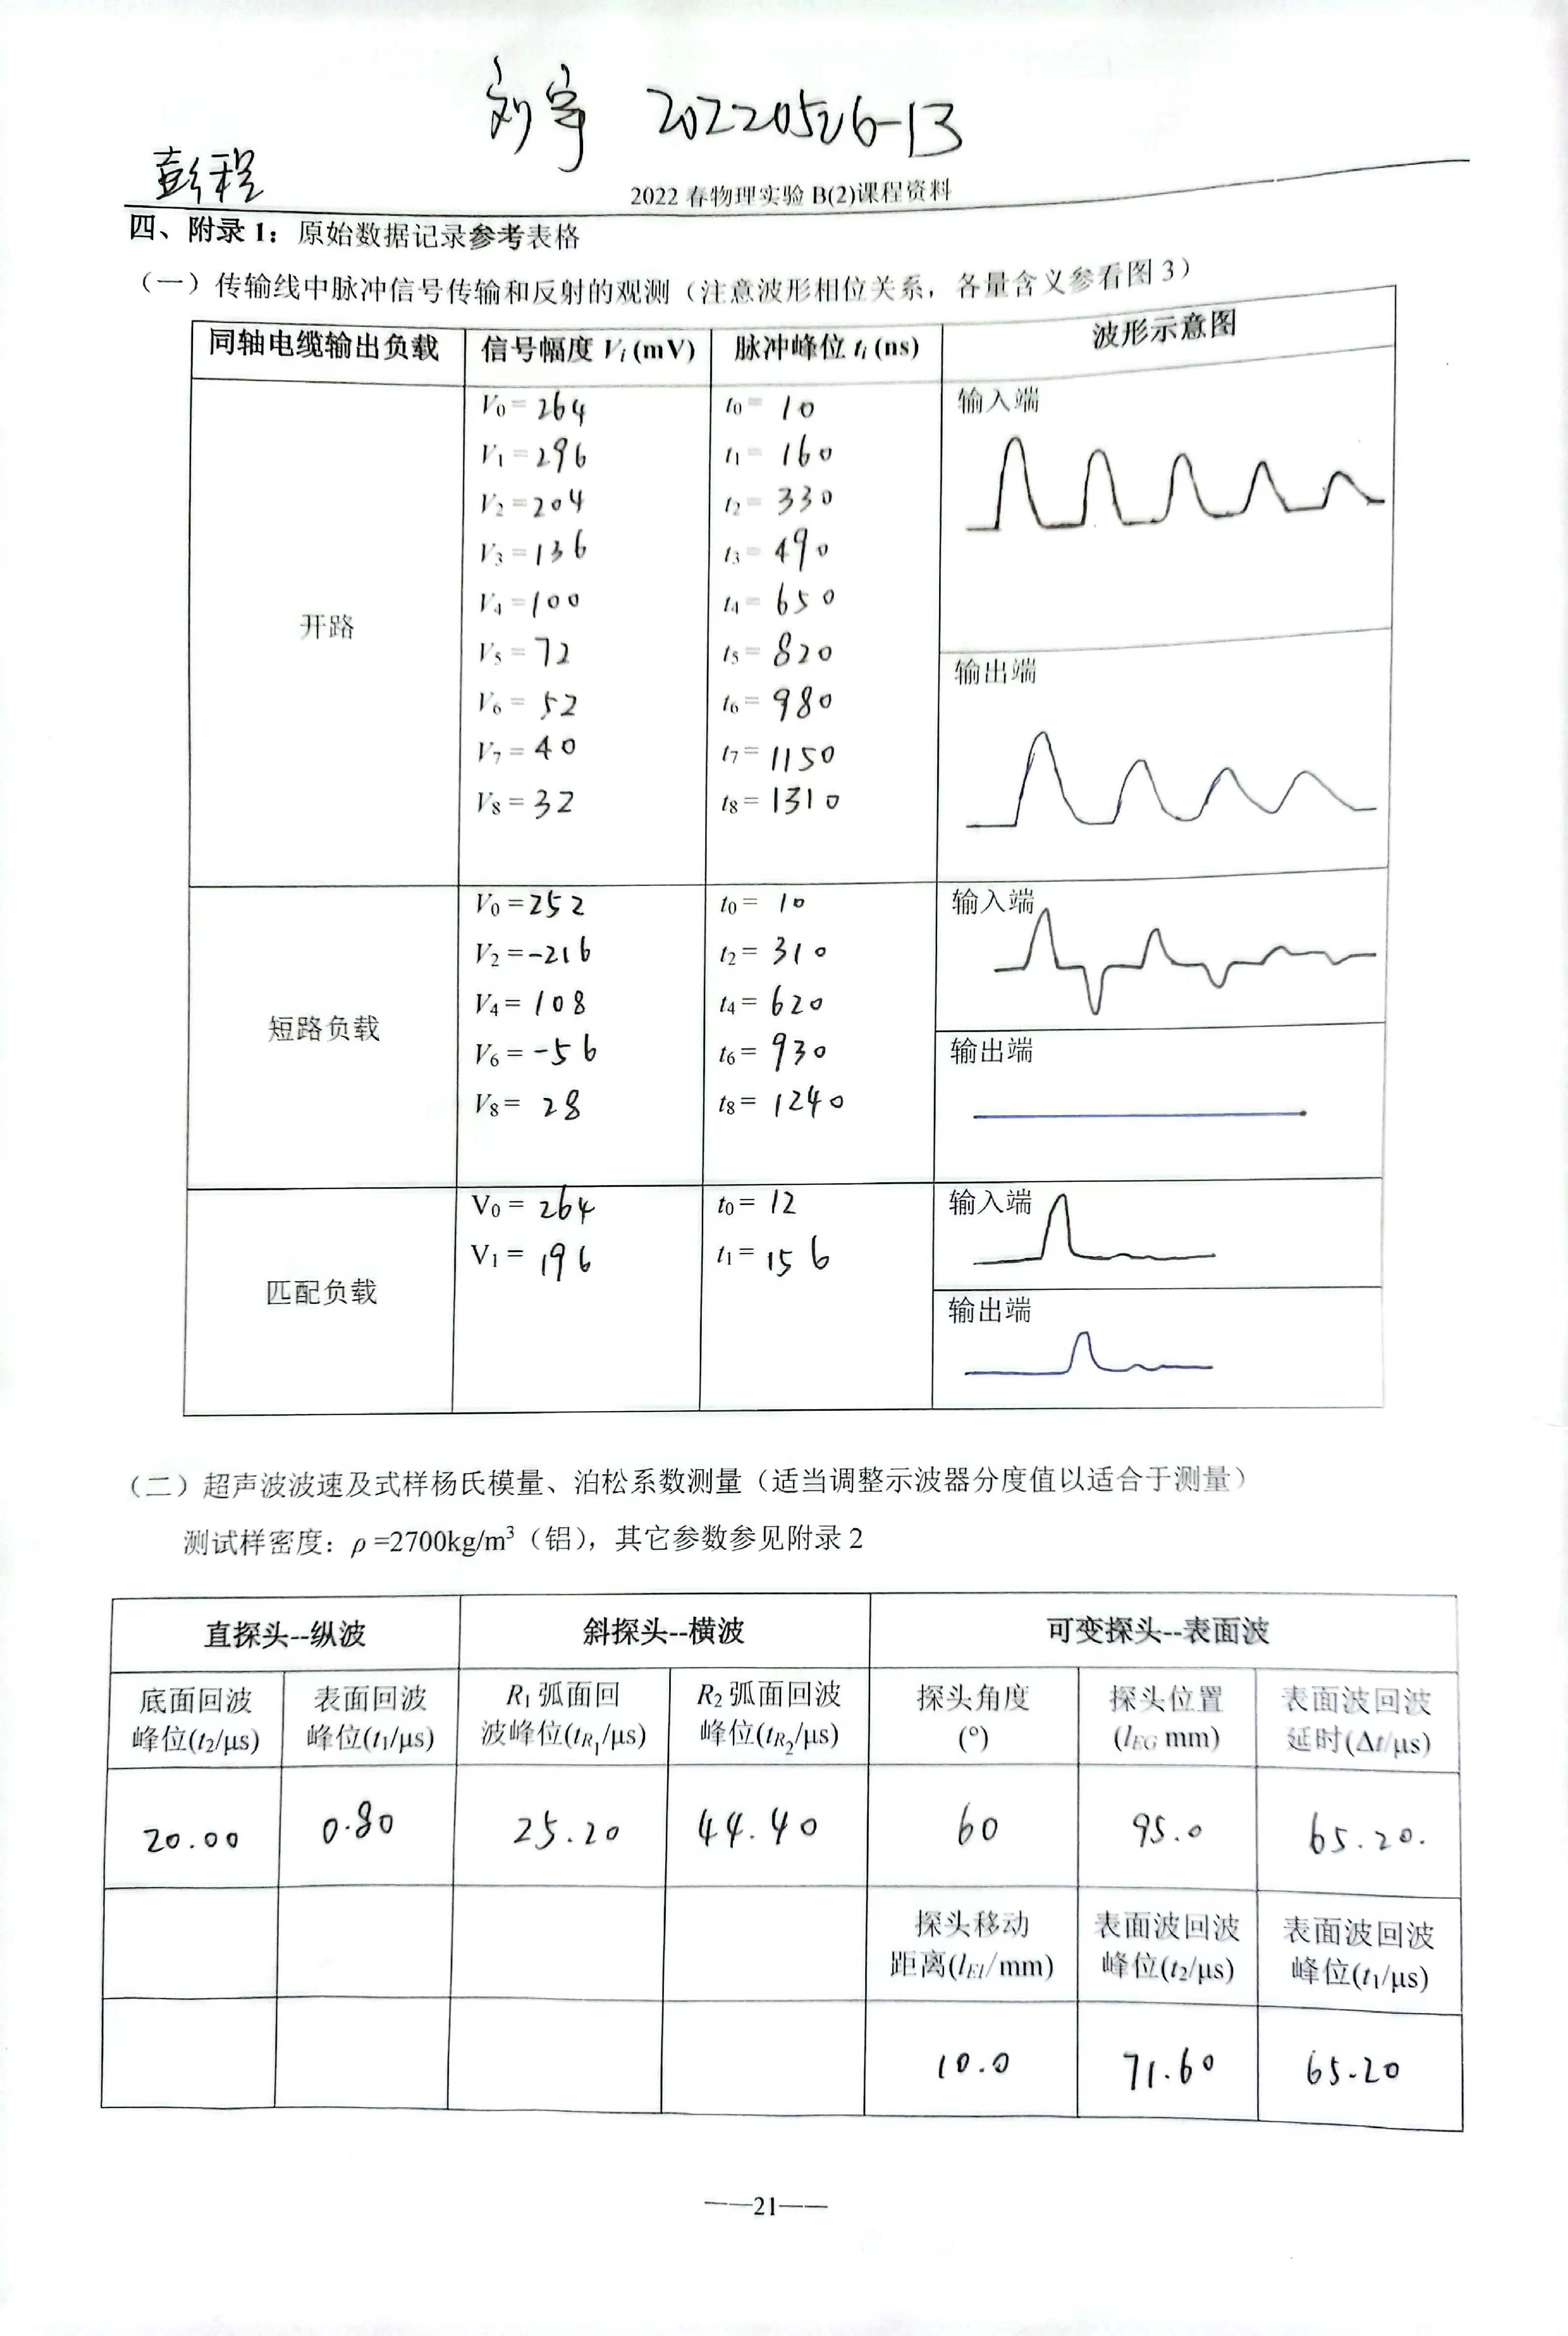
\includegraphics[scale=0.13]{记录1.jpg}
\end{figure}

\begin{figure}[H]
  \centering
  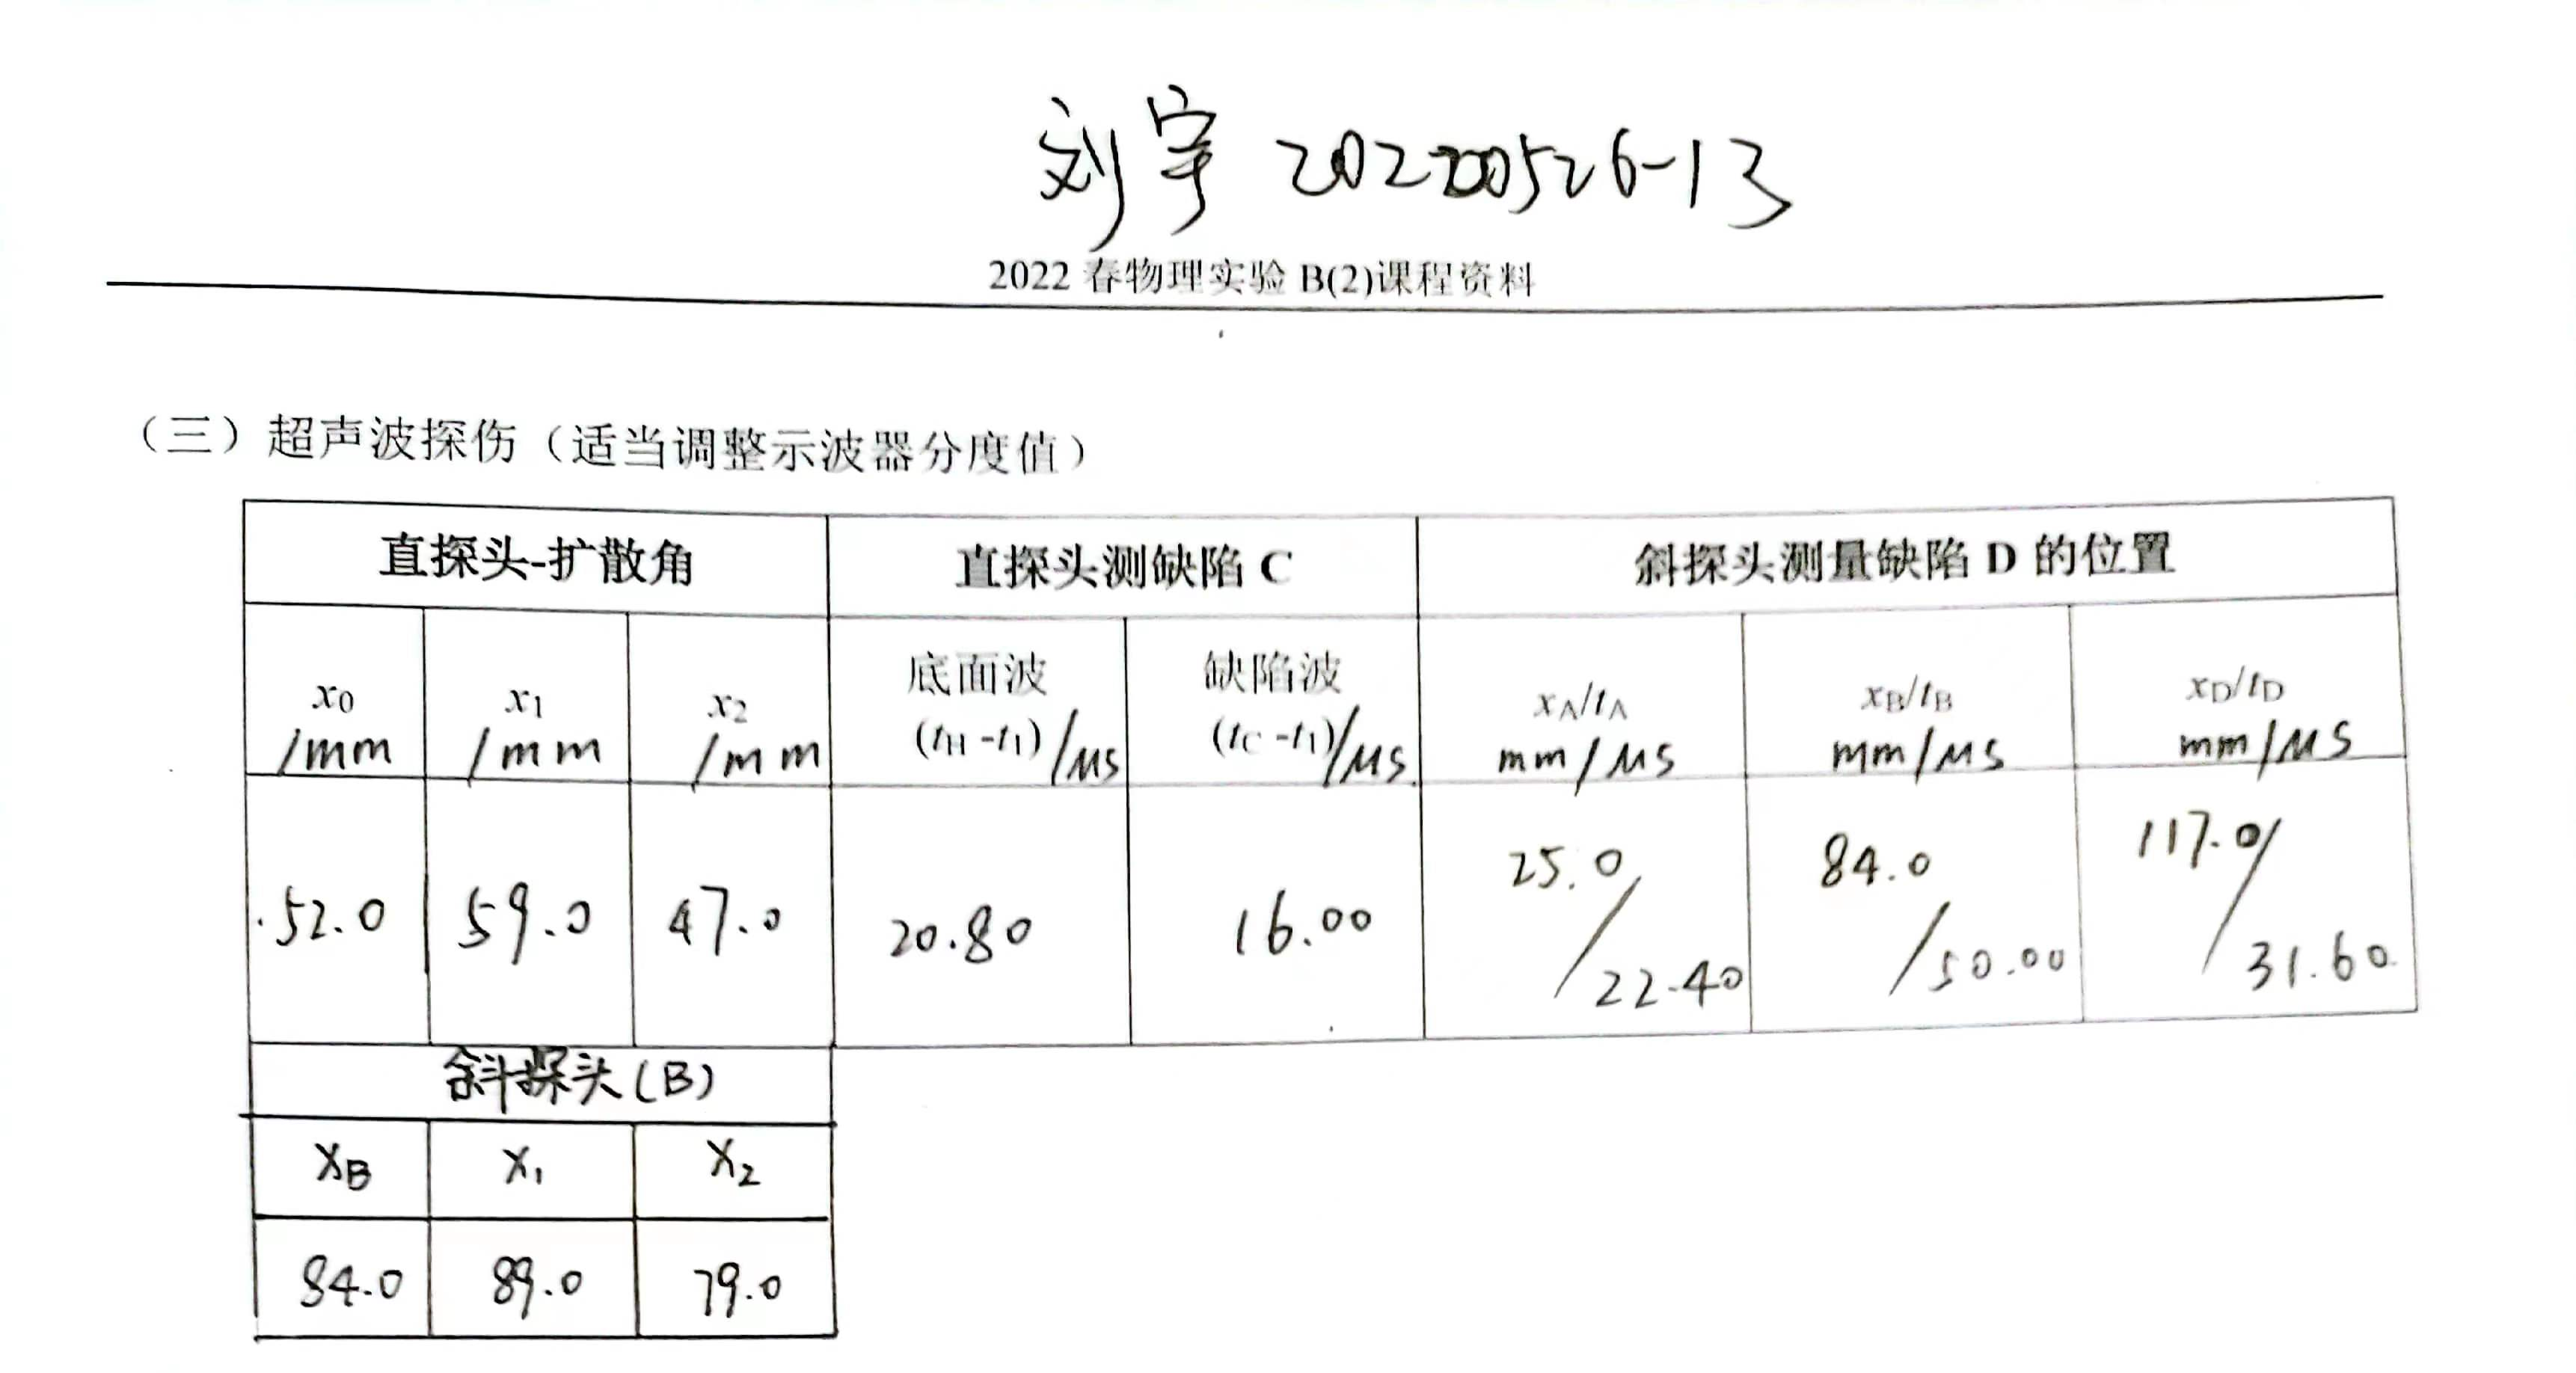
\includegraphics[scale=0.13]{记录2.jpg}
\end{figure}


\end{document}